
\documentclass[conference]{IEEEtran}
\renewcommand\IEEEkeywordsname{Keywords}
\usepackage{array}
\usepackage{tabu}
\usepackage{multirow}

\usepackage{graphicx}
\ifCLASSINFOpdf
\else
\fi
\usepackage{algorithmic}
%\usepackage[options ]{algorithm2e}
\usepackage[ruled,linesnumbered]{algorithm2e}
\makeatletter
\newcommand{\removelatexerror}{\let\@latex@error\@gobble}
\makeatother
\newcommand{\var}{\texttt}
\usepackage{float}
\usepackage{fixltx2e}
\usepackage{stfloats}
\usepackage{tabularx,ragged2e,booktabs,caption}
\usepackage{graphicx}
\usepackage[export]{adjustbox}
\makeatletter
\def\algbackskip{\hskip-\ALG@thistlm}
\makeatother
\hyphenation{op-tical net-works semi-conduc-tor}


\begin{document}

\title{EFFICIENT TASK ALLOCATION STRATEGIES FOR WSNs}


\author{\IEEEauthorblockN{C.Cara Evangeline}
\IEEEauthorblockA{Department of CSE\\
NIT Andhra Pradesh, India\\
Email:caraevangeline10@gmail.com}
\and
\IEEEauthorblockN{C.Kushala}
\IEEEauthorblockA{Department of CSE\\
NIT Andhra Pradesh, India\\
Email:kushi134@gmail.com}
\and
\IEEEauthorblockN{BKSP Kumar Raju Alluri}
\IEEEauthorblockA{Department of CSE\\
NIT Andhra Pradesh, India\\
Email:pavan0712@gmail.com}}
\maketitle
\IEEEpeerreviewmaketitle



\begin{abstract} 
Tasks for wireless sensor networks have severe time and energy constraints. Performance of a sensor network like energy consumption and lifetime is largely affected based on the task allocated to the nodes in a network. This paper presents an efficient task allocation framework for sensor networks. It is generally known that multiple sensor nodes collaborating with each other to perform tasks are an important means of energy balancing. Therefore in this paper, we propose two task allocation strategies which when compared with current related works is much more realistic and efficient for complex task processing in terms of shortening execution time. \\
\begin{IEEEkeywords}
Task Allocation, Resource based sequence task allocation(RBSTA), Quantum based task allocation(QBTA), Energy, Queue length.
\end{IEEEkeywords}
\end{abstract}
\section{INTRODUCTION}
\par In recent years, WSNs have been widely used in many applications including military, industrial, household, medical, marine and other fields, especially in natural disaster monitoring, early warning, rescuing and other emergency situations. This paper presents higher real-time measures such as energy and queue length for task allocation.
\par Task allocation is essential to allocate the workload of each task to proper nodes in an efficient manner. Multiple measures including task execution time, energy consumption, queue length and resources required by tasks are considered as a whole to achieve the best overall performance. 
\subsection{Problem Definition}
\par Many task allocation methods have been proposed for WSNs. Most of them only concentrate on reducing energy consumption of sensor nodes.  However, queue length is not taken into consideration which is an important factor for allocation of tasks.
\par Instead of allocating a task based on energy alone, we take into consideration resources such as CPU cycles, memory (buffer size) and energy. Based on these resources, the proposed approach constructs an allocation table using which the task assignment is completed.
\subsection{Our Approach}
\par It is difficult for a single sensor node to independently accomplish a complex task. Therefore, assigning a complex task to appropriate sensor nodes has become a pressing issue in WSNs. In this paper, we resolve the problem of assigning complex tasks using the proposed algorithm QBTA (Quantum Based Task Allocation) which efficiently allocates the task to multiple nodes based on energy, queue length and time quantum.
%\begin{figure}[H]
%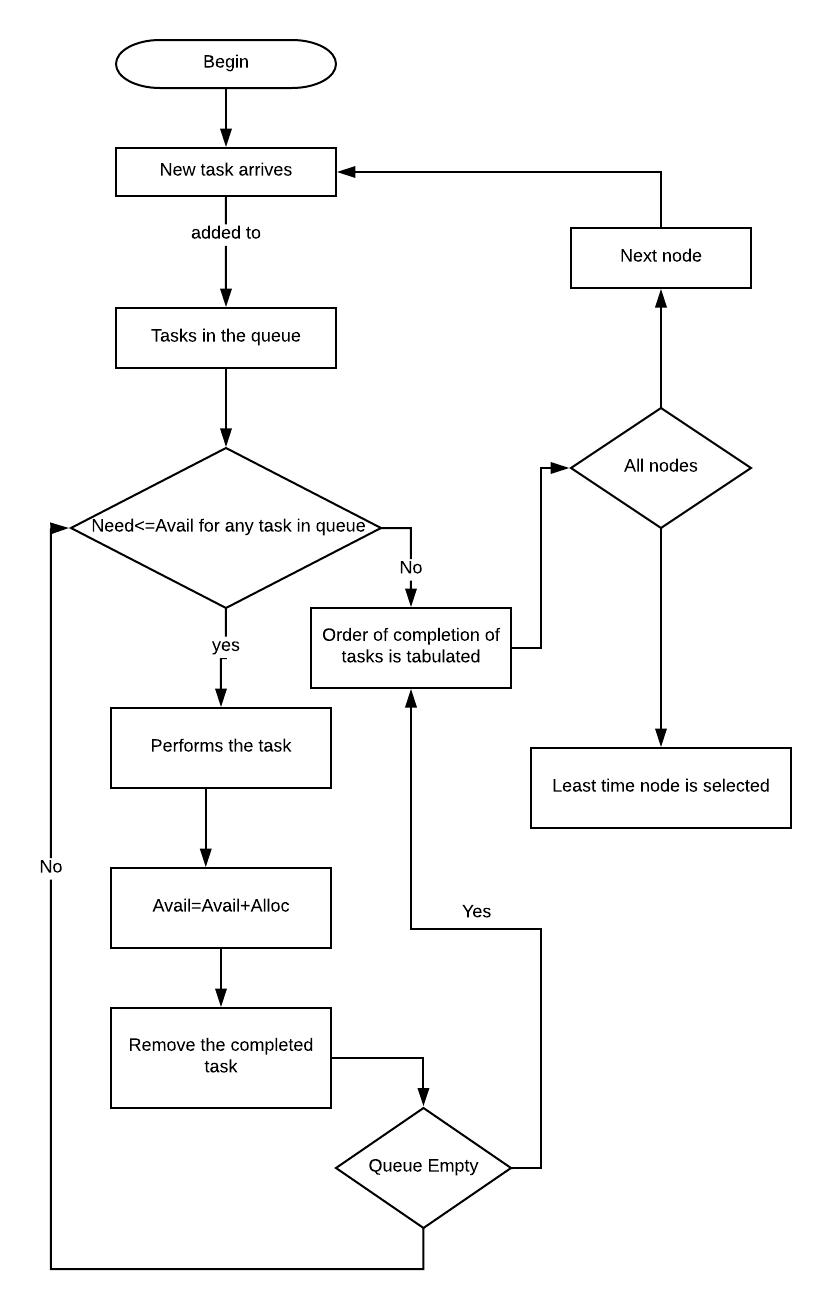
\includegraphics[width=\linewidth]{RBSTA.png}
%  \caption{RBSTA flow chart}
%  \label{fig:1}
%\end{figure}


\par It is generally known that sensor nodes in WSNs are small with limited processing and computing resources. An algorithm RBSTA (Resource Based Sequence for Task Allocation) is also proposed to efficiently allocate a task to a node in WSN.  
%\begin{figure}[H]
%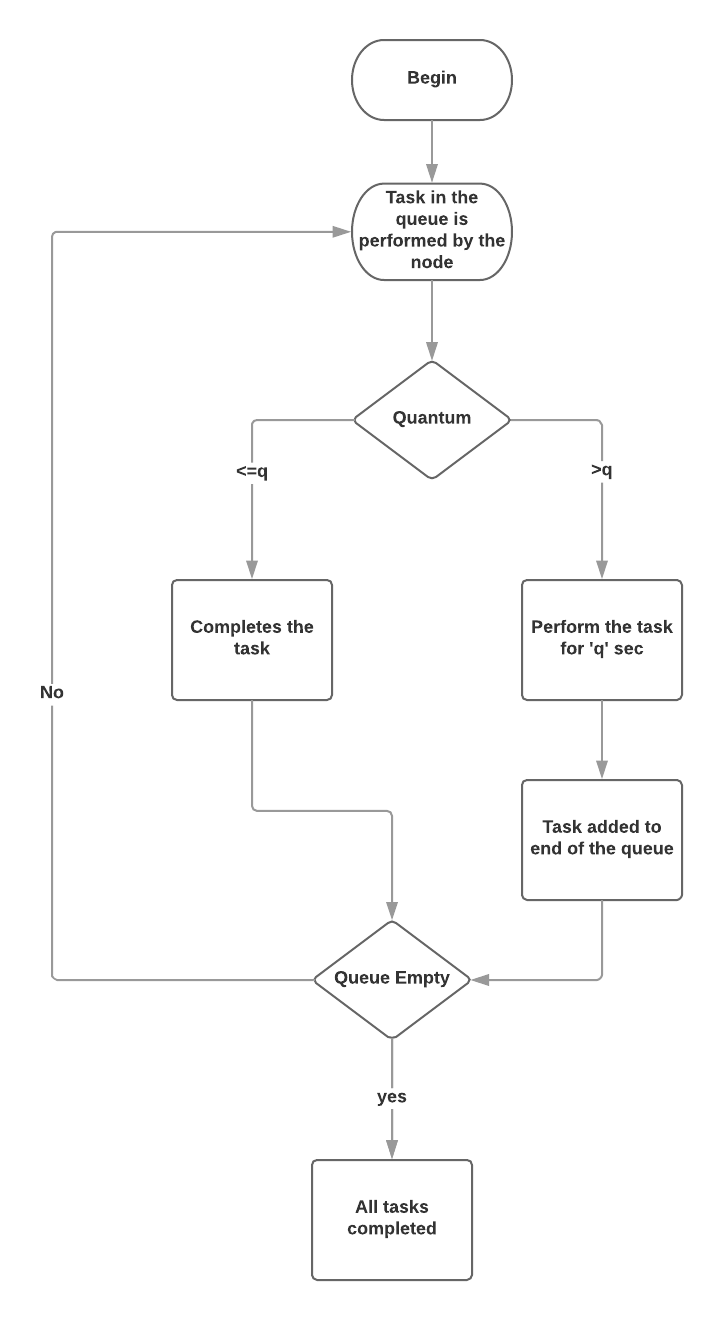
\includegraphics[width=\linewidth]{QBTA.png}
%  \caption{QBTA flow chart}
%  \label{fig:2}
%\end{figure}

\par  Section II contains Related work and comparison with our work. Section III consists of our proposed algorithms (QBTA and RBSTA) along with the other comparison algorithms and graphs. Tables and the Tools used are discussed in Section IV and a summary of our paper is presented in Section V.

\section{RELATED WORK}
\par In recent years, numerous studies have been conducted for task allocation and scheduling. For example, Giannecchini et al[1] proposed an online task scheduling mechanism called CoRAl[1] to dynamically reconfigure a sensor network whenever a new intruder is detected. Given the amount of available resources and the task set, CoRAl determines the sampling frequency for all the tasks so that the frequencies of the tasks on each sensor are optimized subject to the previously evaluated upper-bound execution frequencies. CoRAl does not address mapping tasks to sensor nodes.
\par In, an energy-constrained task mapping and scheduling EcoMapS[3] is proposed. It incorporates channel modeling, concurrent task mapping, communication and computation scheduling, and sensor failure handling algorithm. First, a channel model is presented for singlehop WSNs[3]. Then, based on this channel model, communication and computation are jointly scheduled in the initialization phase. Furthermore, a quick recovery algorithm is executed in the quick recovery phase in case of sensor node failures. However, the guarantee of execution deadline is not provided by EcoMapS, hence it is not suitable for real-time applications. It has not considered queue length parameter which is a required real time factor.
\par Shehory[9], proposed an efficient distributed algorithms with low ratio bounds and with low computational complexities. These properties are proven theoretically and supported by simulations. They are based on both the algorithmic aspects of combinatorics and approximation algorithms for NP-hard problems. First, an approach to agent coalition was proposed where each agent must be a member of only one coalition. Next, this approach is extended for overlapping coalitions. In this paper, we propose approaches for the same with improved reality.  
\par From the above-mentioned related works, we can find that existing task allocation strategies always takes only one influencing factor such as energy consumption or network load or network lifetime into account for task allocation. However, other contributing factors such as queue length, resources cannot be neglected. Therefore, a novel distributed and energy efficient task allocation strategy is proposed.
\section{PROPOSED APPROACH}
\subsection{Allocation of single task based on Energy and Queue Length}
\par Considering energy factor, we allocate a task to the node with highest energy. When only energy is considered, the task gets allocated to a set of nodes.
\par When both energy and queue length are considered, the task gets allocated to different or same set of nodes based on queue length. Figure 1 and 2 shows the difference.\\
\begin{figure}[H]
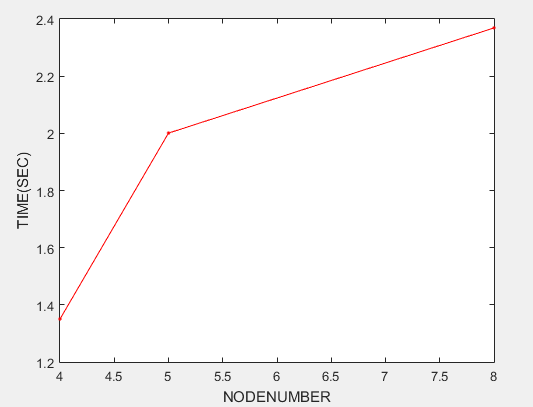
\includegraphics[width= 7cm,frame,center]{fig3.png}
 
  \caption{Task allocation based on energy}
  \label{fig:1}
\end{figure}

\begin{figure}[H]
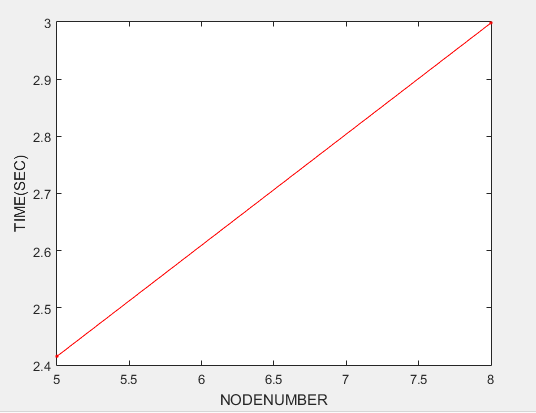
\includegraphics[width=7cm,frame,center]{fig4.png}
  \caption{Task allocation based on energy and Queue Length}
  \label{fig:2}
\end{figure}

The mapping of single task to multiple nodes is achieved through the following steps:
\par i. Until the task gets completed the workload is shared\par  between nodes
\par ii. If the node with highest energy has full buffer size then\par the task is given to next highest energy node.\\
 This process repeats until the assigned task gets completed.
%\par The mapping of single task to multiple nodes is done by using above procedure.


\subsection{Allocation of multiple tasks based on Energy and Queue length}
Two different methodologies were proposed.\\
%\subsubsection{Arriving tasks waits for the task in the queue to complete if the queue is full}
%\par Here the newly arriving task is given highest priority and the time taken to complete the tasks by the node is noted.\\
%\par i. Every node has energy and tasks in its queue.
%\par ii. Priorities are given to task based on the actual time the\par task takes to complete. Task with highest priority has less\par burst time.
%\par iii. Till the tasks gets completed the procedure is repeated.
%\par iv. Task with less time is given to highest energy node. If\par the highest energy node is full, then the newly arriving task\par waits for the last task in the node's queue to complete if\par the last task in the queue has burst time\textless  threshold otherwise\par the task moves on to next highest energy node.
%\par All the newly arriving tasks gets completed and the result of completion time which includes waiting time was tabulated. 
%\begin{figure}[H]
%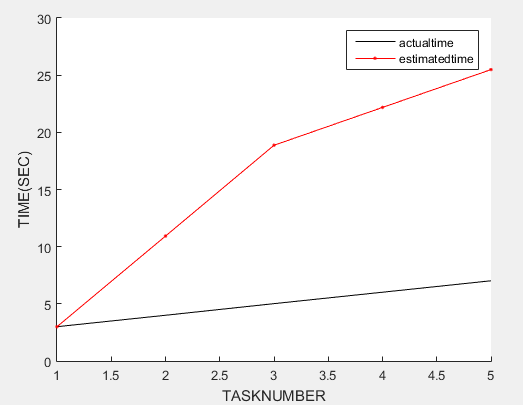
\includegraphics[width=7cm,frame,center]{fig5.png}
%  \caption{Multiple task allocation}
%  \label{fig:5}
%\end{figure}
% 
%The Figure 5 shows the actual time of the tasks and its estimated time when it waits for a task in the queue. The estimated time of completion is drastically higher.\\

\subsubsection{Allocation based on First come first served(FCFS)}
Initially, when all new tasks arrives, they are prioritized based on their execution time (ie.Shortest task is given highest priority). The task which has highest priority is given to highest energy node. Similarly, other tasks are mapped based on their priorities. Each node has n tasks in its queue. The tasks are performed in the order in which they are placed in the queue. 

\begin{figure}[H]
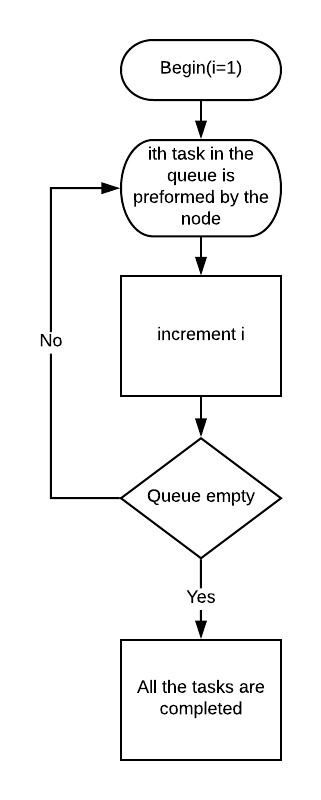
\includegraphics[width=4cm,center]{FCFS.png}
  \caption{FCFS Flow Chart}
  \label{fig:6}
\end{figure}

Figure 3 describes the order in which each task in a queue is performed by a node.\\
% \par i. Every node has energy and tasks in its queue.
% \par ii. Priorities are given to task based on the actual time the\par task takes to complete. Task with highest priority has less\par burst time.
% \par iii. Till all the tasks gets completed the procedure is\par repeated.
% \par iv. The task with the highest priority is given to highest\par energy node.
% \par v. Now, all the tasks in its queue are performed based on\par the order in which the tasks are in the queue.
% \par vi. So, the new task completion time will be including the\par previous tasks completion time.
%  \par vii. The above procedure is repeated till all the new tasks\par are completed.
% \par The task completion time is tabulated.\\
\subsubsection{Allocation based on time Quantum(QBTA)}
Multiple tasks arrives and the tasks are prioritized based on their execution time. Now, highest priority task is performed by the highest energy node. Similarly, all the newly arriving tasks are allotted to each node based on task priority. Every node contains n tasks in its queue. Based on time quantum(q), a task is performed for q seconds and then added to the end of the queue. This is done till all tasks in the queue are completed. The procedure is followed for all newly arriving tasks.
\begin{figure}[H]
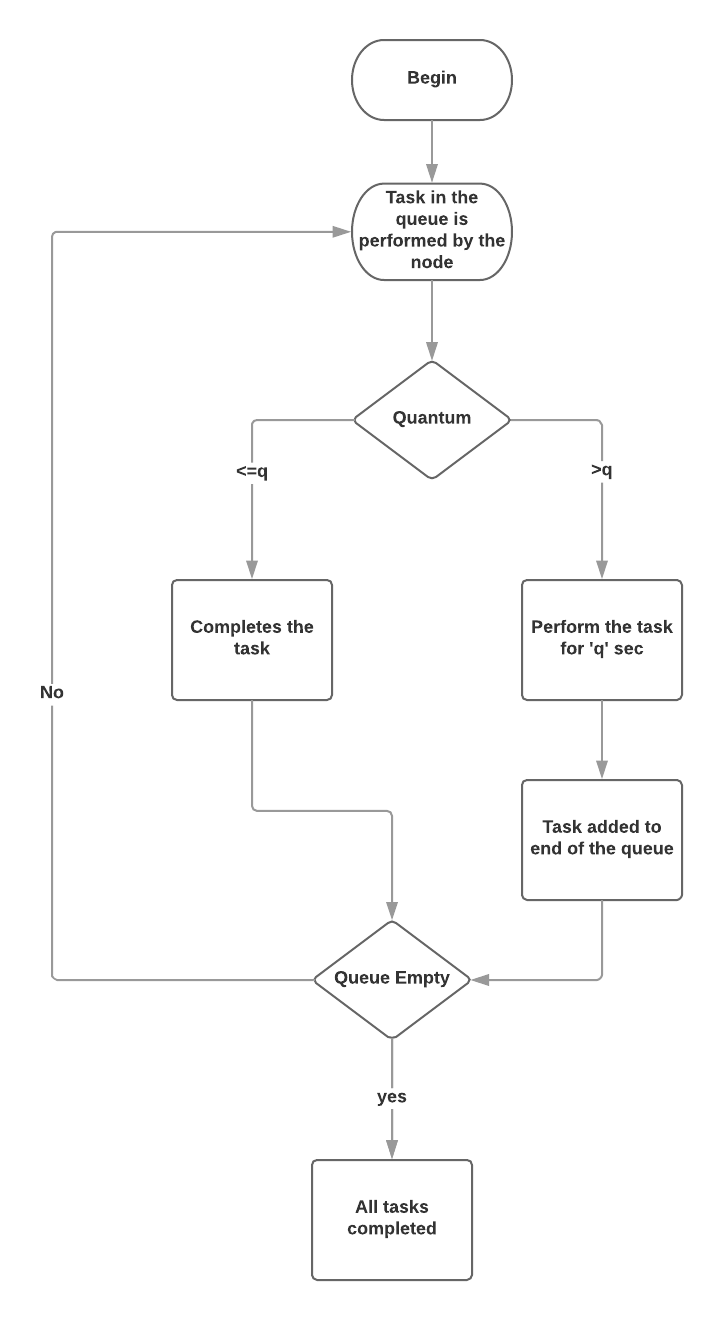
\includegraphics[width=\linewidth]{QBTA.png}
  \caption{QBTA flow chart}
  \label{fig:2}
\end{figure}

Figure 4 describes the order in which each task in a queue is performed by a node. QBTA procedure is described in Algorithm 1. In FCFS Algorithm, newly arriving task will be placed at the end of a queue which increases task completion time whereas in QBTA algorithm every task in a queue is performed for q seconds and placed at the end of the queue which decreases the task completion time. The difference in the efficiency of FCFS and QBTA is shown in Figure 5. 
\begin{algorithm}
\SetAlgoLined
 \KwData{Energy, Queue length of each node and all the t tasks burst time bt}
 \KwResult{Time for completion of all the tasks }
  %buffersize=15\;
  i=1 \;
 \While{i\textless=t}{
Find the $ith$ maximum energy node and allocate the task which requires $ith$ least time \;
// Every node has previously allocated tasks and some nodes have newly arrived  tasks 
}
i=1 \; 
q=2  //Time Quantum \;
 \While{i\textless=t}{
 Select the node which got the newly allocated task 
 \While{Until completion of all tasks in the Queue}{
 % read current\;
  \eIf{task has bt\textless =q}{
  task will leave after completion \;
  node will perform next task in its queue \;
  }
  {
  task is performed by the node for q seconds and then placed at the end of its queue \;
  Now,node performs the next task in the queue \;
  } 
    }
  $ct[i] \leftarrow completion\_time$ \; 
   }
  \Return ct[] \; 
 \caption{ QBTA(Quantum Based Task Allocation)}
\end{algorithm}
\begin{figure}[H]
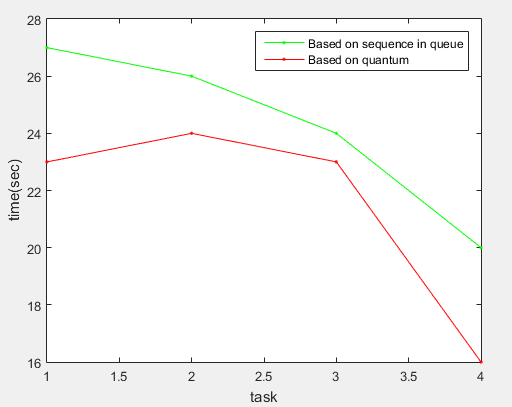
\includegraphics[width=7cm,frame,center]{fig6.png}
  \caption{Multiple task allocation}
  \label{fig:6}
\end{figure}



%\par Figure 6 shows that QBTA is efficient algorithm for multiple task allocation.

\subsection{Allocation of task based on sequence table}
In the previous proposed approach, tasks are allotted to a node based on energy and queue length. In RBSTA algorithm, before giving a newly arriving task to a node, the completion time of the tasks when given to all nodes individually is calculated and the node which performs the task in less time is the efficient node to perform the arrived task. Considering multiple measures (ie. resources such as CPU cycles, energy and queue length) here a sequence table is constructed based on the sequence obtained by RBSTA algorithm. Through the sequence, completion time of newly arriving task for each node is known. Similar to routing algorithm where packet is transferred to the next node which is at shortest distance from the source node, in RBSTA the task is given to the efficient node which performs the newly arrived task in less time.

\begin{figure}[H]
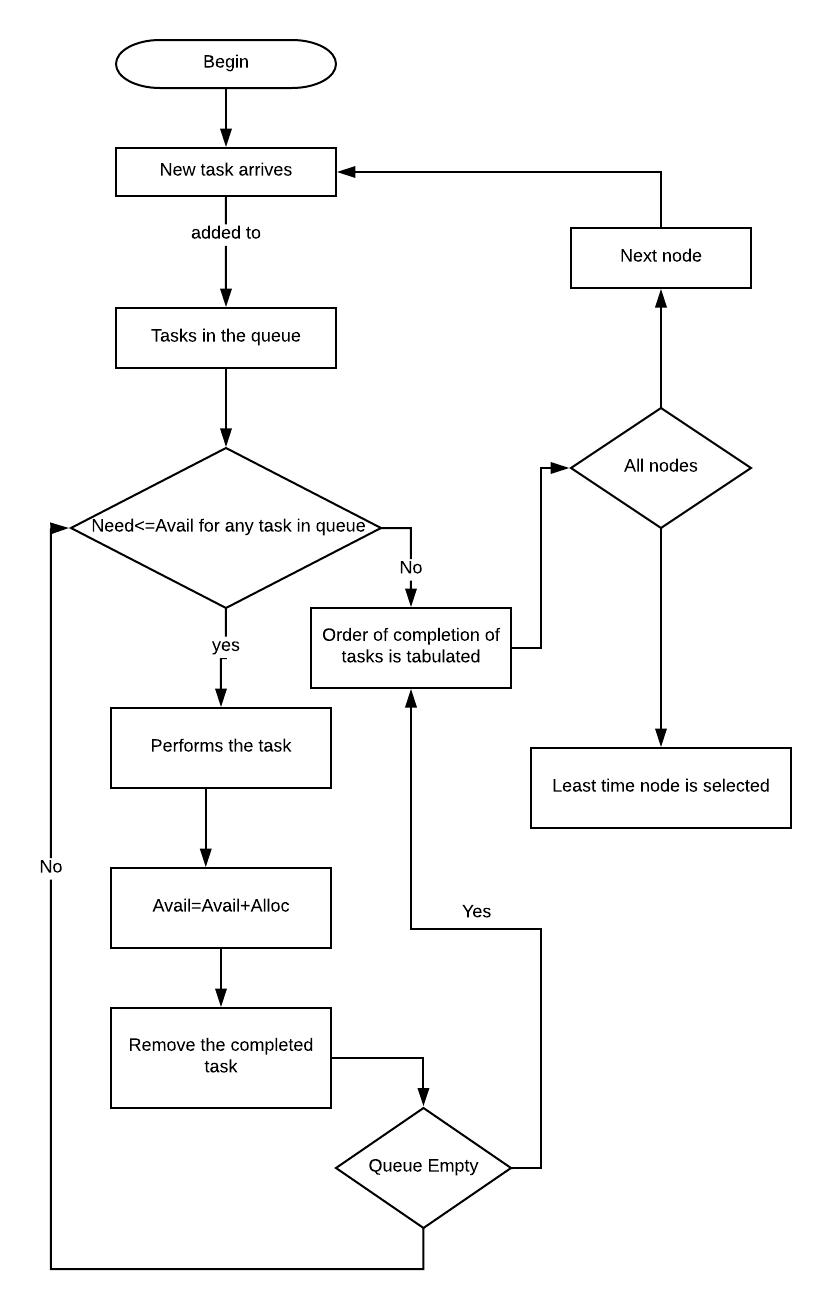
\includegraphics[width=\linewidth]{RBSTA.png}
  \caption{RBSTA flow chart}
  \label{fig:1}
\end{figure}

Figure 6 describes the flow of RBSTA Algorithm. RBSTA procedure is described in Algorithm 2.
\begin{algorithm}%[H]
\SetAlgoLined
 \KwData{Resources required for newly arriving task(max)}
 \KwResult{Efficient node for performing a given task}
  %buffersize=15\;
  i=1 \;
  j=1 \;
 \While{i\textless= n}{
$max[][]\leftarrow maximum\_ resources\_of\_ tasks\_ in\_ queue()$ \;
$alloc[][]\leftarrow allocated\_ resources\_ of\_ tasks\_ in\_ queue()$ \;
 
 //Add the maximum resources of the newly arriving tasks to max[][] and append  [0,0,0] to alloc[][] \; 
%\While{j\textless= no of tasks in Queue of n+1}{
$avail[]\leftarrow free\_ resources\_ of\_ $ith$\_ node$ \;
need[][]=max[][]-alloc[][] \;
\While{Until all tasks in the queue of $ith$ node gets checked}{
\eIf{need[][]\textless= avail[]}{
Complete the task \;
avail[]=avail[]+alloc[][] \;
}{
check for the next task \;
}
 }
$sequence\leftarrow order\_ of\_ tasks\_ completion$ \; 
}
Based on the sequence table, time for newly arriving task for each node is calculated \; 

 % read current\;
 % \eIf{}{
  
  
 %  }
 
%   }
  \Return min\_ time\_ node()  \; 
 \caption{RBSTA(Resource Based Sequence for Task Allocation)}
 
\end{algorithm}


\section{EXPERIMENTAL RESULTS}
The proposed algorithms were tested in simulation in a Matlab framework. MATLAB (matrix laboratory) is a multi-paradigm numerical computing environment.

\par Table 1 shows the dependence of allocation of task on Queue length which the existing works failed to consider. Efficient way of allocating a task based on time quantum is shown in Table 2. Table 3 is the sequence table from which we can get the efficient node to perform a task.
\begin {table}[H]
% \resizebox{0.9\textwidth}{!}{\begin{minipage}{\textwidth}
 \captionof{table}{Single task shared between nodes} \label{tab:title}
 \begin{center}
\begin{tabular}{ |c|c|c|c|c| } 
%\captionof{table}{Table Title} \label{tab:title}
\hline
Nodenumber & Energy & Queue length &  E & E and QL \\
\hline
 1 & 0.4709 & 7  &  \textendash & \textendash \\ 
 2 & 0.1948 & 4  & \textendash & \textendash \\ 
 3 & 0.2277 & 8 &  \textendash & \textendash \\
 4 & 0.9234 & 15 & yes  & \textendash \\
 5 & 0.9049 & 6 & yes & yes\\
 6 & 0.1111 & 11 & \textendash& \textendash  \\
 7 & 0.5949 & 10 &\textendash & \textendash \\
 8 & 0.7112 & 14 & yes & yes \\
 9 & 0.2967 & 13 & \textendash & \textendash \\
 10 & 0.5079 & 9 & \textendash & \textendash \\ 
\hline
\end{tabular}
\end{center}
%\end{minipage}}
\end{table}
 From table 1, it is known that when a node with highest energy has full buffer size, then the task is allocated to other nodes.



\begin {table}[H]
% \resizebox{0.9\textwidth}{!}{\begin{minipage}{\textwidth}
 \captionof{table}{Comparision between FCFS and QBTA} \label{tab:title}
 \begin{center}
\begin{tabular}{ |c|c|c|c|c| } 
%\captionof{table}{Table Title} \label{tab:title}
\hline
 Task number & Burst Time & FCFS CT & QBTA CT \\
\hline
 1 & 2.9983 & 27 & 23   \\ 
 2 & 3.9999 & 26 & 24  \\ 
 3 & 5.0169 & 24 & 23  \\
 4 & 6.0162 & 20 & 16 \\

\hline
\end{tabular}
\end{center}
%\end{minipage}}
\end{table}

From table 2, QBTA is giving a more efficient result when compared to FCFS algorithm. 



\begin {table}[H]
% \resizebox{0.9\textwidth}{!}{\begin{minipage}{\textwidth}
 \captionof{table}{RBSTA Sequence Table} \label{tab:title}
 \begin{center}
\begin{tabular}{ |c|c|c|c|c|c|c|c|c| } 
%\captionof{table}{Table Title} \label{tab:title}
\hline
Node & QL & s1 & s2 & s3 & s4 & s5 & s6 & Time \\
\hline
1 & 6 & T4 & T2 & T1 & T3 & T5 & T6 & 15  \\ 
2 & 6 & T1 & T2 & T3 & T4 & T5 & T6 & 11   \\
3 & 2 & \textendash & \textendash & \textendash  & \textendash & \textendash & \textendash &  \textendash \\
4 & 6 & T2 & T3 & T4 & T1 & T5 & T6 & 16\\
5 & 5 & T1 & T2 & T4 & T3 & T5 & \textendash & 9 \\
\hline
\end{tabular}
\end{center}
%\end{minipage}}
\end{table}
Similar to Routing table, a sequence table is constructed based on which task can be allocated to a node which completes it in less time. From Table 3 we can infer that task is allocated to node 5 since it performs the task in less time while compared to other nodes. 

\par Hence, Table 1 shows the dependence of task allocation on Queue Length, from Table 2 we can infer that Quantum based task allocation is efficient and Table 3 gives the efficient node to which a task can  be allocated.

\section{Conclusion}
In this paper, we introduced two efficient task allocation approaches which are implemented based on parameters like energy, queue length and the resources available. From the experimental results, it is observed that the proposed approaches optimized the energy consumption and decreased the execution time.


\bibliographystyle{IEEEtran}

\bibliography{IEEEabrv,../bib/paper}

\begin{thebibliography}{1}
\bibitem{}
Giannecchini, Simone, Marco Caccamo, and Chi-Sheng Shih. "Collaborative resource allocation in wireless sensor networks." Real-Time Systems, 2004. ECRTS 2004. Proceedings. 16th Euromicro Conference on. IEEE, 2004.
\bibitem{}
Gerkey, Brian P., and Maja J. Matarić. "A formal analysis and taxonomy of task allocation in multi-robot systems." The International Journal of Robotics Research 23.9 (2004): 939-954.
\bibitem{}
Tian, Yuan, Eylem Ekici, and Fusun Ozguner. "Energy-constrained task mapping and scheduling in wireless sensor networks." Mobile Adhoc and Sensor Systems Conference, 2005. IEEE International Conference on. IEEE, 2005.
\bibitem{}
Younis, Mohamed, Kemal Akkaya, and Anugeetha Kunjithapatham. "Optimization of task allocation in a cluster-based sensor network." Computers and Communication, 2003.(ISCC 2003). Proceedings. Eighth IEEE International Symposium on. IEEE, 2003.
\bibitem{}
Botelho, Sylvia C., and Rachid Alami. "M+: a scheme for multi-robot cooperation through negotiated task allocation and achievement." Robotics and Automation, 1999. Proceedings. 1999 IEEE International Conference on. Vol. 2. IEEE, 1999.
\bibitem{}
Edalat, Neda, Chen-Khong Tham, and Wendong Xiao. "An auction-based strategy for distributed task allocation in wireless sensor networks." Computer Communications 35.8 (2012): 916-928.
\bibitem{}
Deng, Yueyue, et al. "Task allocation and path planning for collaborative AUVs operating through an underwater acoustic network." OCEANS 2010. IEEE, 2010.
\bibitem{}
Ferri, Gabriele, et al. "A market-based task allocation framework for autonomous underwater surveillance networks." OCEANS 2017-Aberdeen. IEEE, 2017.
\bibitem{}
Shehory, Onn, and Sarit Kraus. "Methods for task allocation via agent coalition formation." Artificial intelligence 101.1-2 (1998): 165-200.
\bibitem{}
Kang, Qin-Ma, et al. "Task allocation for maximizing reliability of distributed computing systems using honeybee mating optimization." Journal of Systems and Software 83.11 (2010): 2165-2174.
\bibitem{}
Yu, Yang, and Viktor K. Prasanna. "Energy-balanced task allocation for collaborative processing in wireless sensor networks." Mobile Networks and Applications 10, no. 1-2 (2005): 115-131.
\end{thebibliography}





\end{document}

